\chapter{Motor Control and Communication}
\label{chap:mcc}

The \ac{MCC} subsystem is responsible for providing sufficient thrust to the airship for its movement and for providing communication with a controller on the ground.
%
\section{Functional and Technical Requirements}
%
\subsection{Functional Requirements}
%What function(s) does the subsystem have to fulfill?
%
Below are listed the primary functional requirements for the \ac{MCC}:
%
\begin{itemize}
\item Reliable communication between ground controller (transmitter) and airship (receiver)
\item Independent speed control for each of the motors to allow control of flight direction
\item Sufficient thrust to propel the airship considering the requirements and flight conditions as discussed in Section \ref{sec:constraints}
\item Operation of the airship from the ground 
\end{itemize}
%
\subsection{Technical Requirements}
%What technical requirements constrain the subsystem design? - e.g. mass, power, strength, stability etc.
%
The technical requirements for the \ac{MCC} subsystem are presented in Table \ref{tab:technical_requirements_mcc}.
%
\begin{table}[H]
\centering
\caption{Technical requirements}
\label{tab:technical_requirements_mcc}
\begin{tabular}{l r}
\hline
\textbf{Parameter} & \textbf{Value}\\ \hline
Total mass & $<250\,g$\\
Input voltage & $6-9.5\,V$\\
Average power consumption & $\sim 45\,W$\\
\hline
\end{tabular}
\end{table}
%
\noindent
As it was decided to use a blimp from Esrange instead of the custom-built \ac{MSE} (see chapter \ref{chap:mse}), the whole system had to be redesigned. The main changes were the increased dimensions of the blimp and the decreased total lift mass. This required for the \ac{MCC} to use more powerful and more efficient motors, since the \ac{EPS} was affected as well. The transmitter/receiver system however remained unchanged.
%
\subsection{Expected Performance}
The expected performance of the chosen \ac{MCC} design is listed in Table \ref{tab:performance_mcc}.
%
\begin{table}[H]
\centering
\caption{Expected performance of motors and controls}
\label{tab:performance_mcc}
\begin{tabular}{l r}
\hline
\textbf{Parameter} & \textbf{Value}\\ \hline
Total mass & $\sim 55\,g$\\
Max. current per motor & $7.5\,A$ \\
Max. motor voltage & $11.2\,V$ \\
Number of motors & $2$ \\
Motor efficiency & $77 \%$ \\ 
Motor RPM & $1400\,RPM/V$\\
Motor dimensions & $27.6 \times 11 mm$ \\
Transmission frequency & $2.4\,GHz$\\
Receiver channels & $6$\\
\hline
\end{tabular}
\end{table}
%
%
\section{Critical Design}
%Explain the preliminary design including block diagrams, schematics, drawings, etc.
%
The functioning of the \ac{MCC} subsystem is shown in Figure \ref{fig:design_block}. The transceiver consists of a $2.4\,GHz$ transmitter and receiver (see below). The receiver forwards the motor speed control commands to the \ac{ESC} which in turn control the motor to reach the desired speed.
%
\begin{figure}[h]
\centering
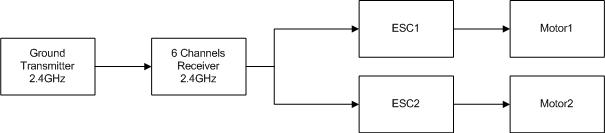
\includegraphics[scale=0.8]{figures/blockdiagram.jpg}
\caption{MCC block diagram}
\label{fig:design_block}
\end{figure}
%
\subsection{Motors, Controllers and Propellers}
%
Brush-less motors are selected as they are known to be powerful, durable and light at the same time. Figure \ref{fig:Motors} shows a motor with propeller and connected to an \ac{ESC}.
%
\begin{figure}[h]
\centering
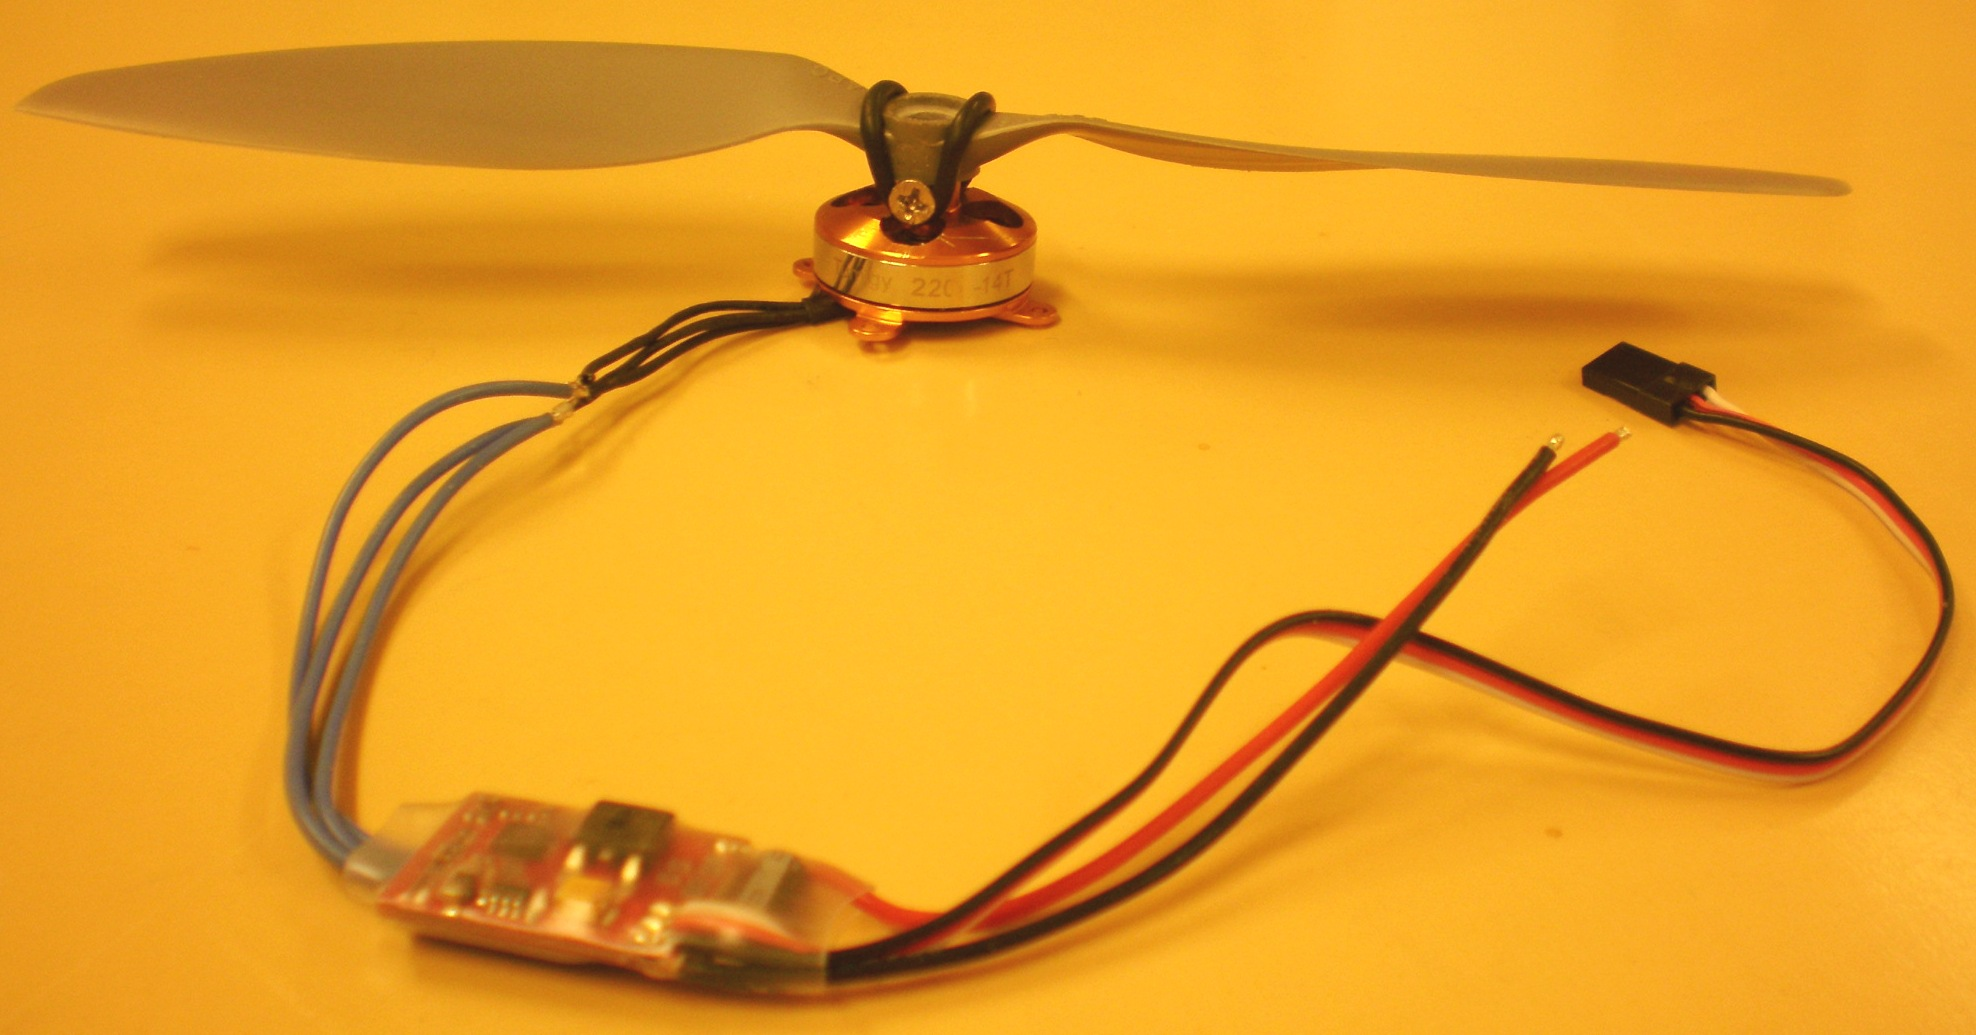
\includegraphics[width=0.8\textwidth]{figures/fig_CDR_MCC_motor_with_propeller_esc.jpg}
\caption{MCC motor with propeller and ESC}
\label{fig:Motors}
\end{figure}
%
%\noindent
The speed of the motor can be controlled by the following methods:
%
\begin{itemize}
\item Use a \ac{COTS} \ac{ESC} for each motor
\item Build a motor speed controller using a microprocessor
\end{itemize}
%
%\noindent
The primary advantage of using \ac{COTS} \ac{ESC}s is the ease of use. This reduces the development cycle to a large extent. The disadvantage of using it is limited scalability i.e. functions like autonomous control and telemetry and telecommanding are not possible. Nevertheless, \ac{COTS} \ac{ESC}s will be used to control the speed of the motors because of time constraints. If time permits it will be desirable to build a speed controller with the help of a microprocessor. The new motors however require a higher current than the motors that were originally selected. Therefore suitable \ac{ESC}s are selected which are able to supply a maximum current of $10\,A$.
%
\subsection{Transceiver System}
%
For the transceiver system the available options are to use
%
\begin{itemize}
\item A $72\,MHz$ transceiver system that uses Amplitude/Frequency Modulation
\item A $2.4\,GHz$ transceiver system that uses Spread Spectrum Technology
\end{itemize}
%
%\noindent
A comparison between these two technologies is shown in Table \ref{tab:transceiver}.
%
\begin{table}
\centering
\caption{Transceiver systems}
\label{tab:transceiver}
\begin{tabular}{|l l l|}
\hline
\textbf{Parameter:} &  \textbf{$2.4\,GHz$ Transceiver} & \textbf{$72\,MHz$ Transceiver}\\ 
\hline
Frequency Used & $2.4\,GHz$ & $72\,MHz$ \\
Crystal Used & No & Yes \\
Change in Frequency & On next power up & By changing the crystal \\
Ability to transmit through obstacles & Weak & Very Good\\
Bandwidth & Wide & Narrow\\
Data Rate & High & Low\\
Power Usage & Less & More\\
RF Noise Immunity & Very Good & Less \\
\hline
\end{tabular}
\end{table}
%\vspace{-2.0em}
%
%\noindent
It is clear from Table \ref{tab:transceiver} that a $2.4\,GHz$ transceiver system is better for the chosen application. The only disadvantage of using a $2.4\,GHz$ transceiver system is that the receiver should have very reliable batteries and the voltage should constantly be maintained at a particular level. The reason is that there are small processors in the transmitter and receiver that carry out many complex calculations every second. These processors require a constant steady supply of current to work properly. If there is an interruption in the supply current of the receiver there will be problems with the communication channel.
\\
\\
The $2.4\,GHz$ transceiver system is selected for the communication channel. The transceiver uses the $2.4\,GHz$ frequency band and the spread spectrum technology for transmission of signals. This feature helps in removing all interfering frequencies caused by other electronic equipments which improves the communication channel. The other major advantage of using spread spectrum technology is that the communication channel is not affected, even when someone is using the same frequency band.
%
\section{Test and Verification}
%
Table \ref{tab:mcc_test} lists completed and scheduled tests of the \ac{MCC} subsystem.
%
\begin{table}[H]
\centering
\caption{MCC test program}
\label{tab:mcc_test}
\begin{tabular}{p{0.25\textwidth}p{0.35\textwidth}p{0.35\textwidth}}
\hline
\textbf{Test} &  \textbf{Description} & \textbf{Status}\\ 
\hline
\rr Motor control from ground transmitter & Two motors should be controlled from the ground transmitter via the onboard receivers and \acp{ESC}. & \rr Completed with success. Some re-programming of ground transmitter is needed to make it more intuitive to use.\tn
Motor thrust measurement & \rr A rack, with the two motors mounted on, is placed on a scale that measures the generated thrust. & \rr Completed, see Figure \ref{fig:motor_thrust_level}. At $\sim 66\,W(\sim 11\,V\;,\;6\,A)$ the motors generated a thrust of $\sim 210\,g\,(2060\,N)$\tn
Communication range & \rr Effective communication range between ground transmitter and onboard receiver should be tested up to at least $250\,m$. & Pending. \tn
\hline
\end{tabular}
\end{table}
%
%
\begin{figure}[bht]
\centering
\begin{minipage}[c]{0.48\textwidth}
\centering
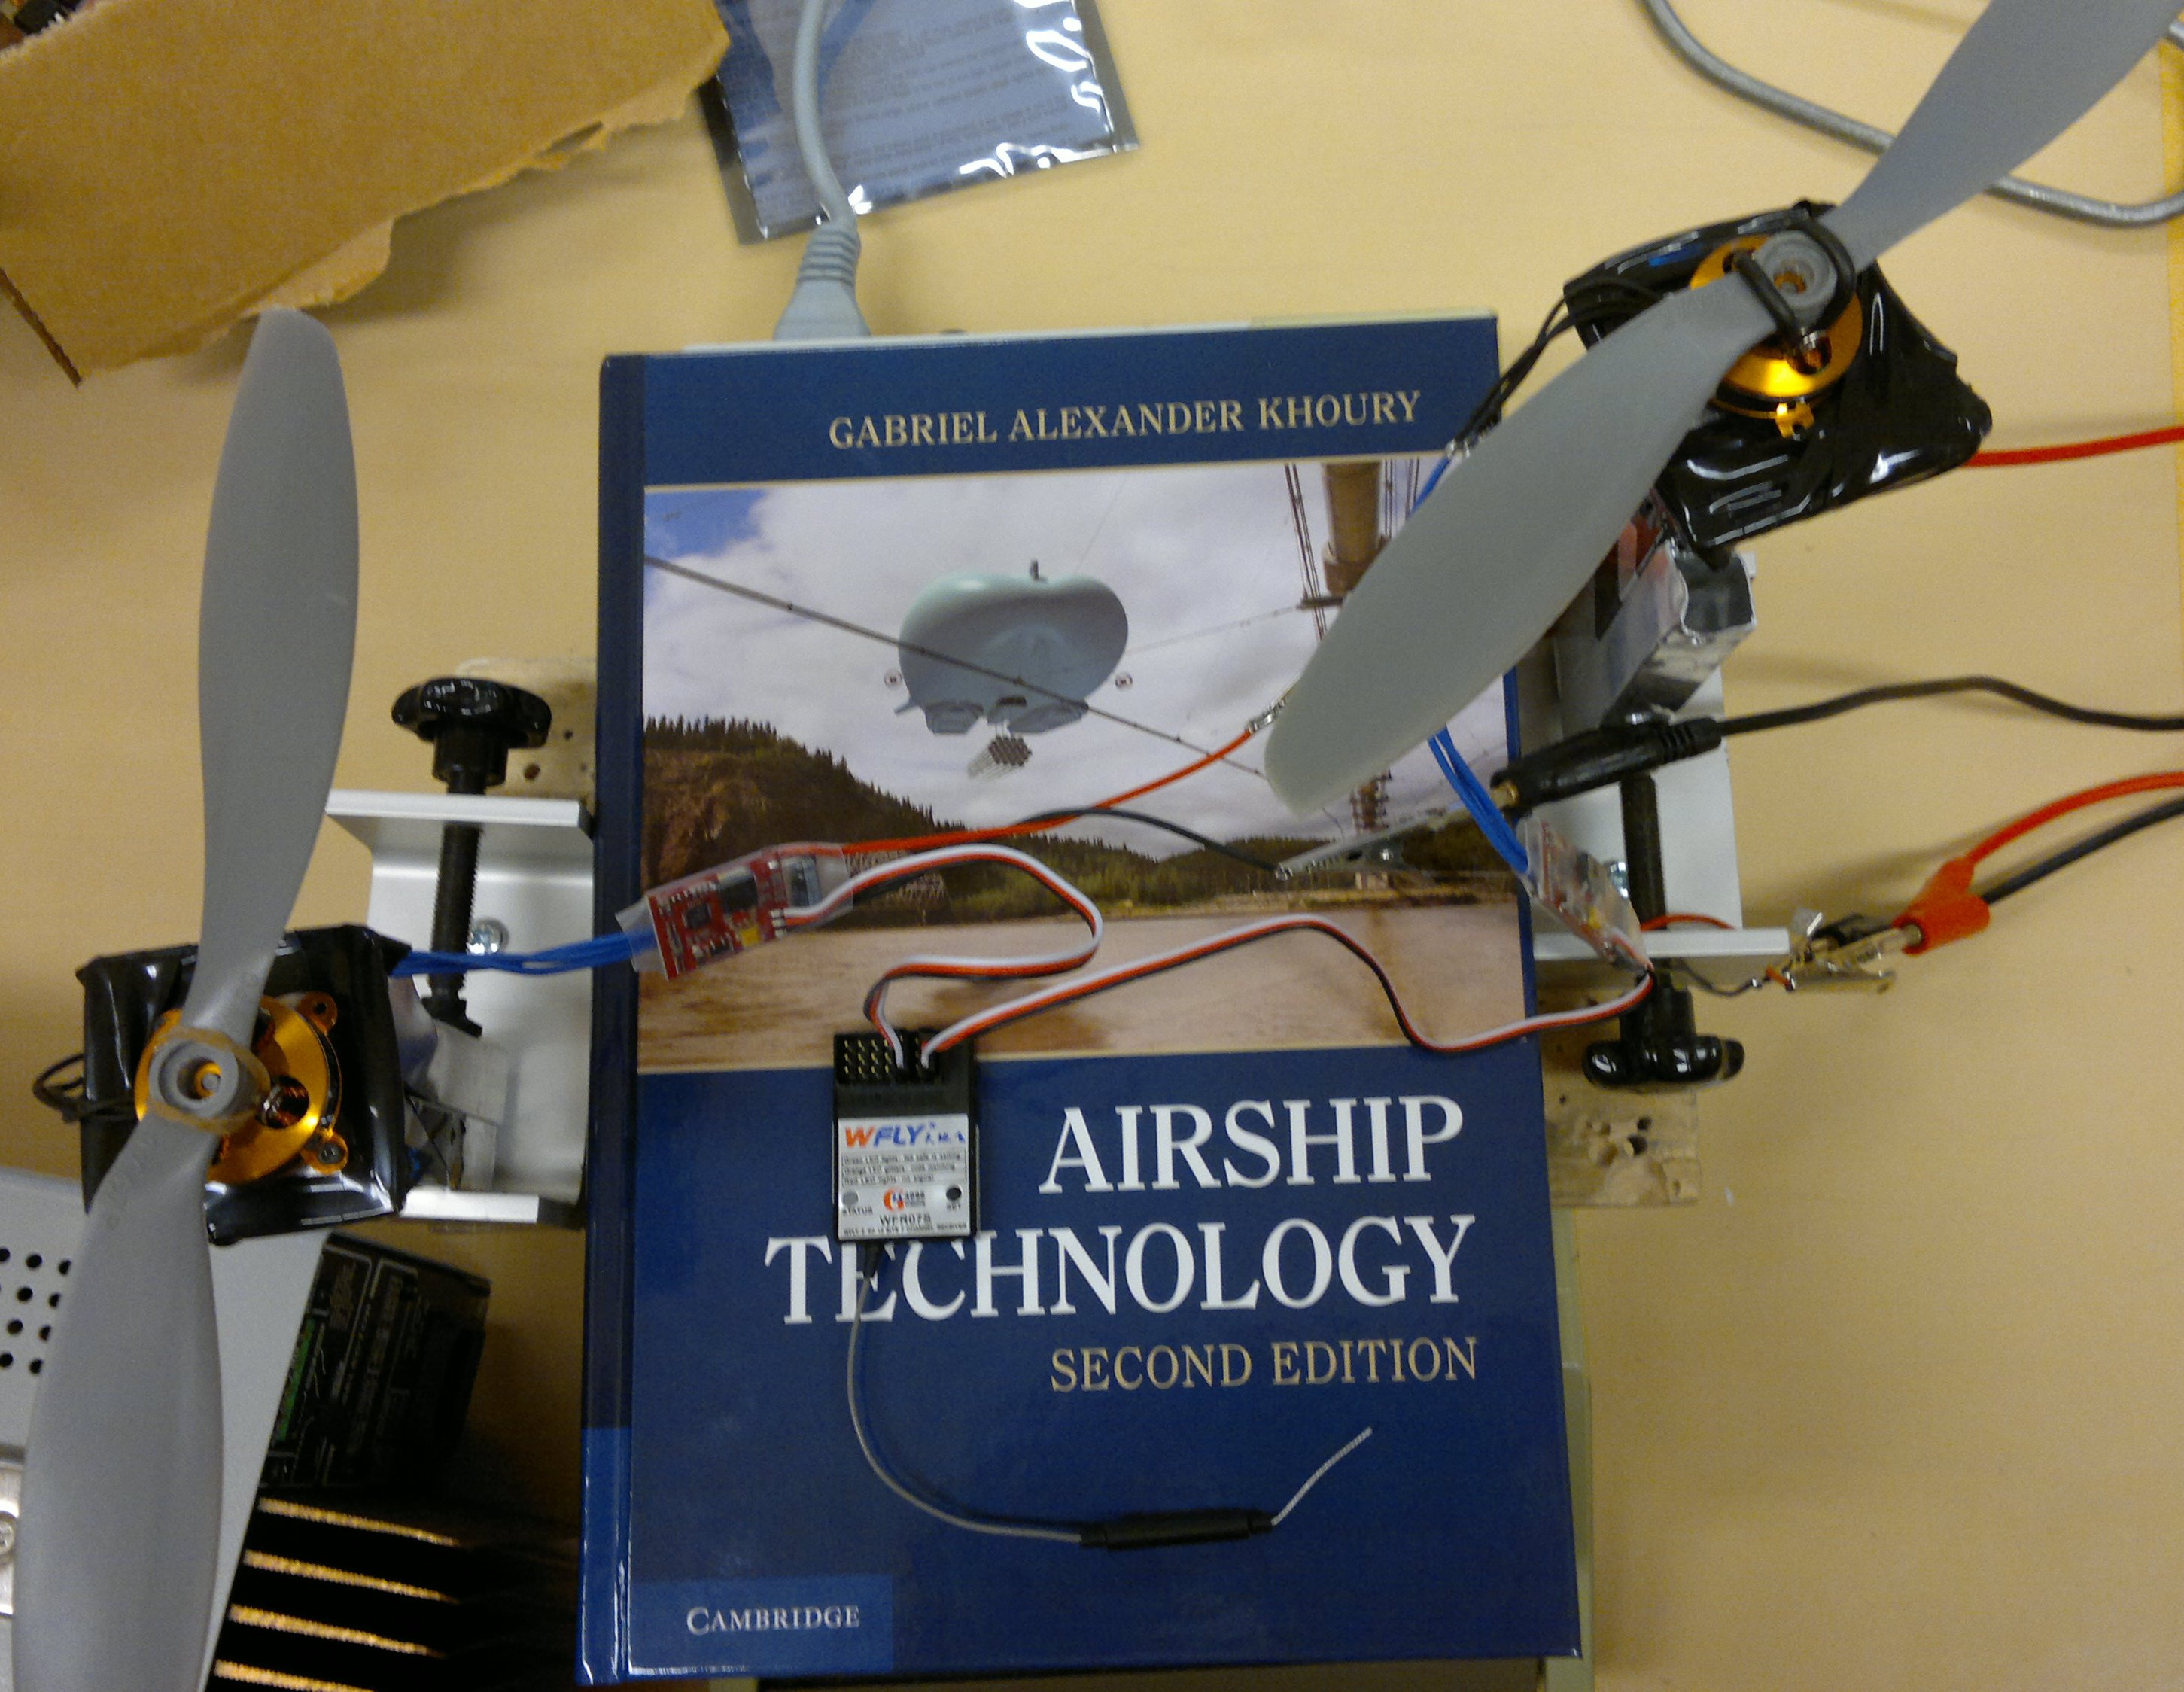
\includegraphics[scale=0.28]{figures/fig_CDR_MCC_motor_thrust_test1.jpg}
\end{minipage}
\vspace{2mm}
\begin{minipage}[c]{0.48\textwidth}
\centering
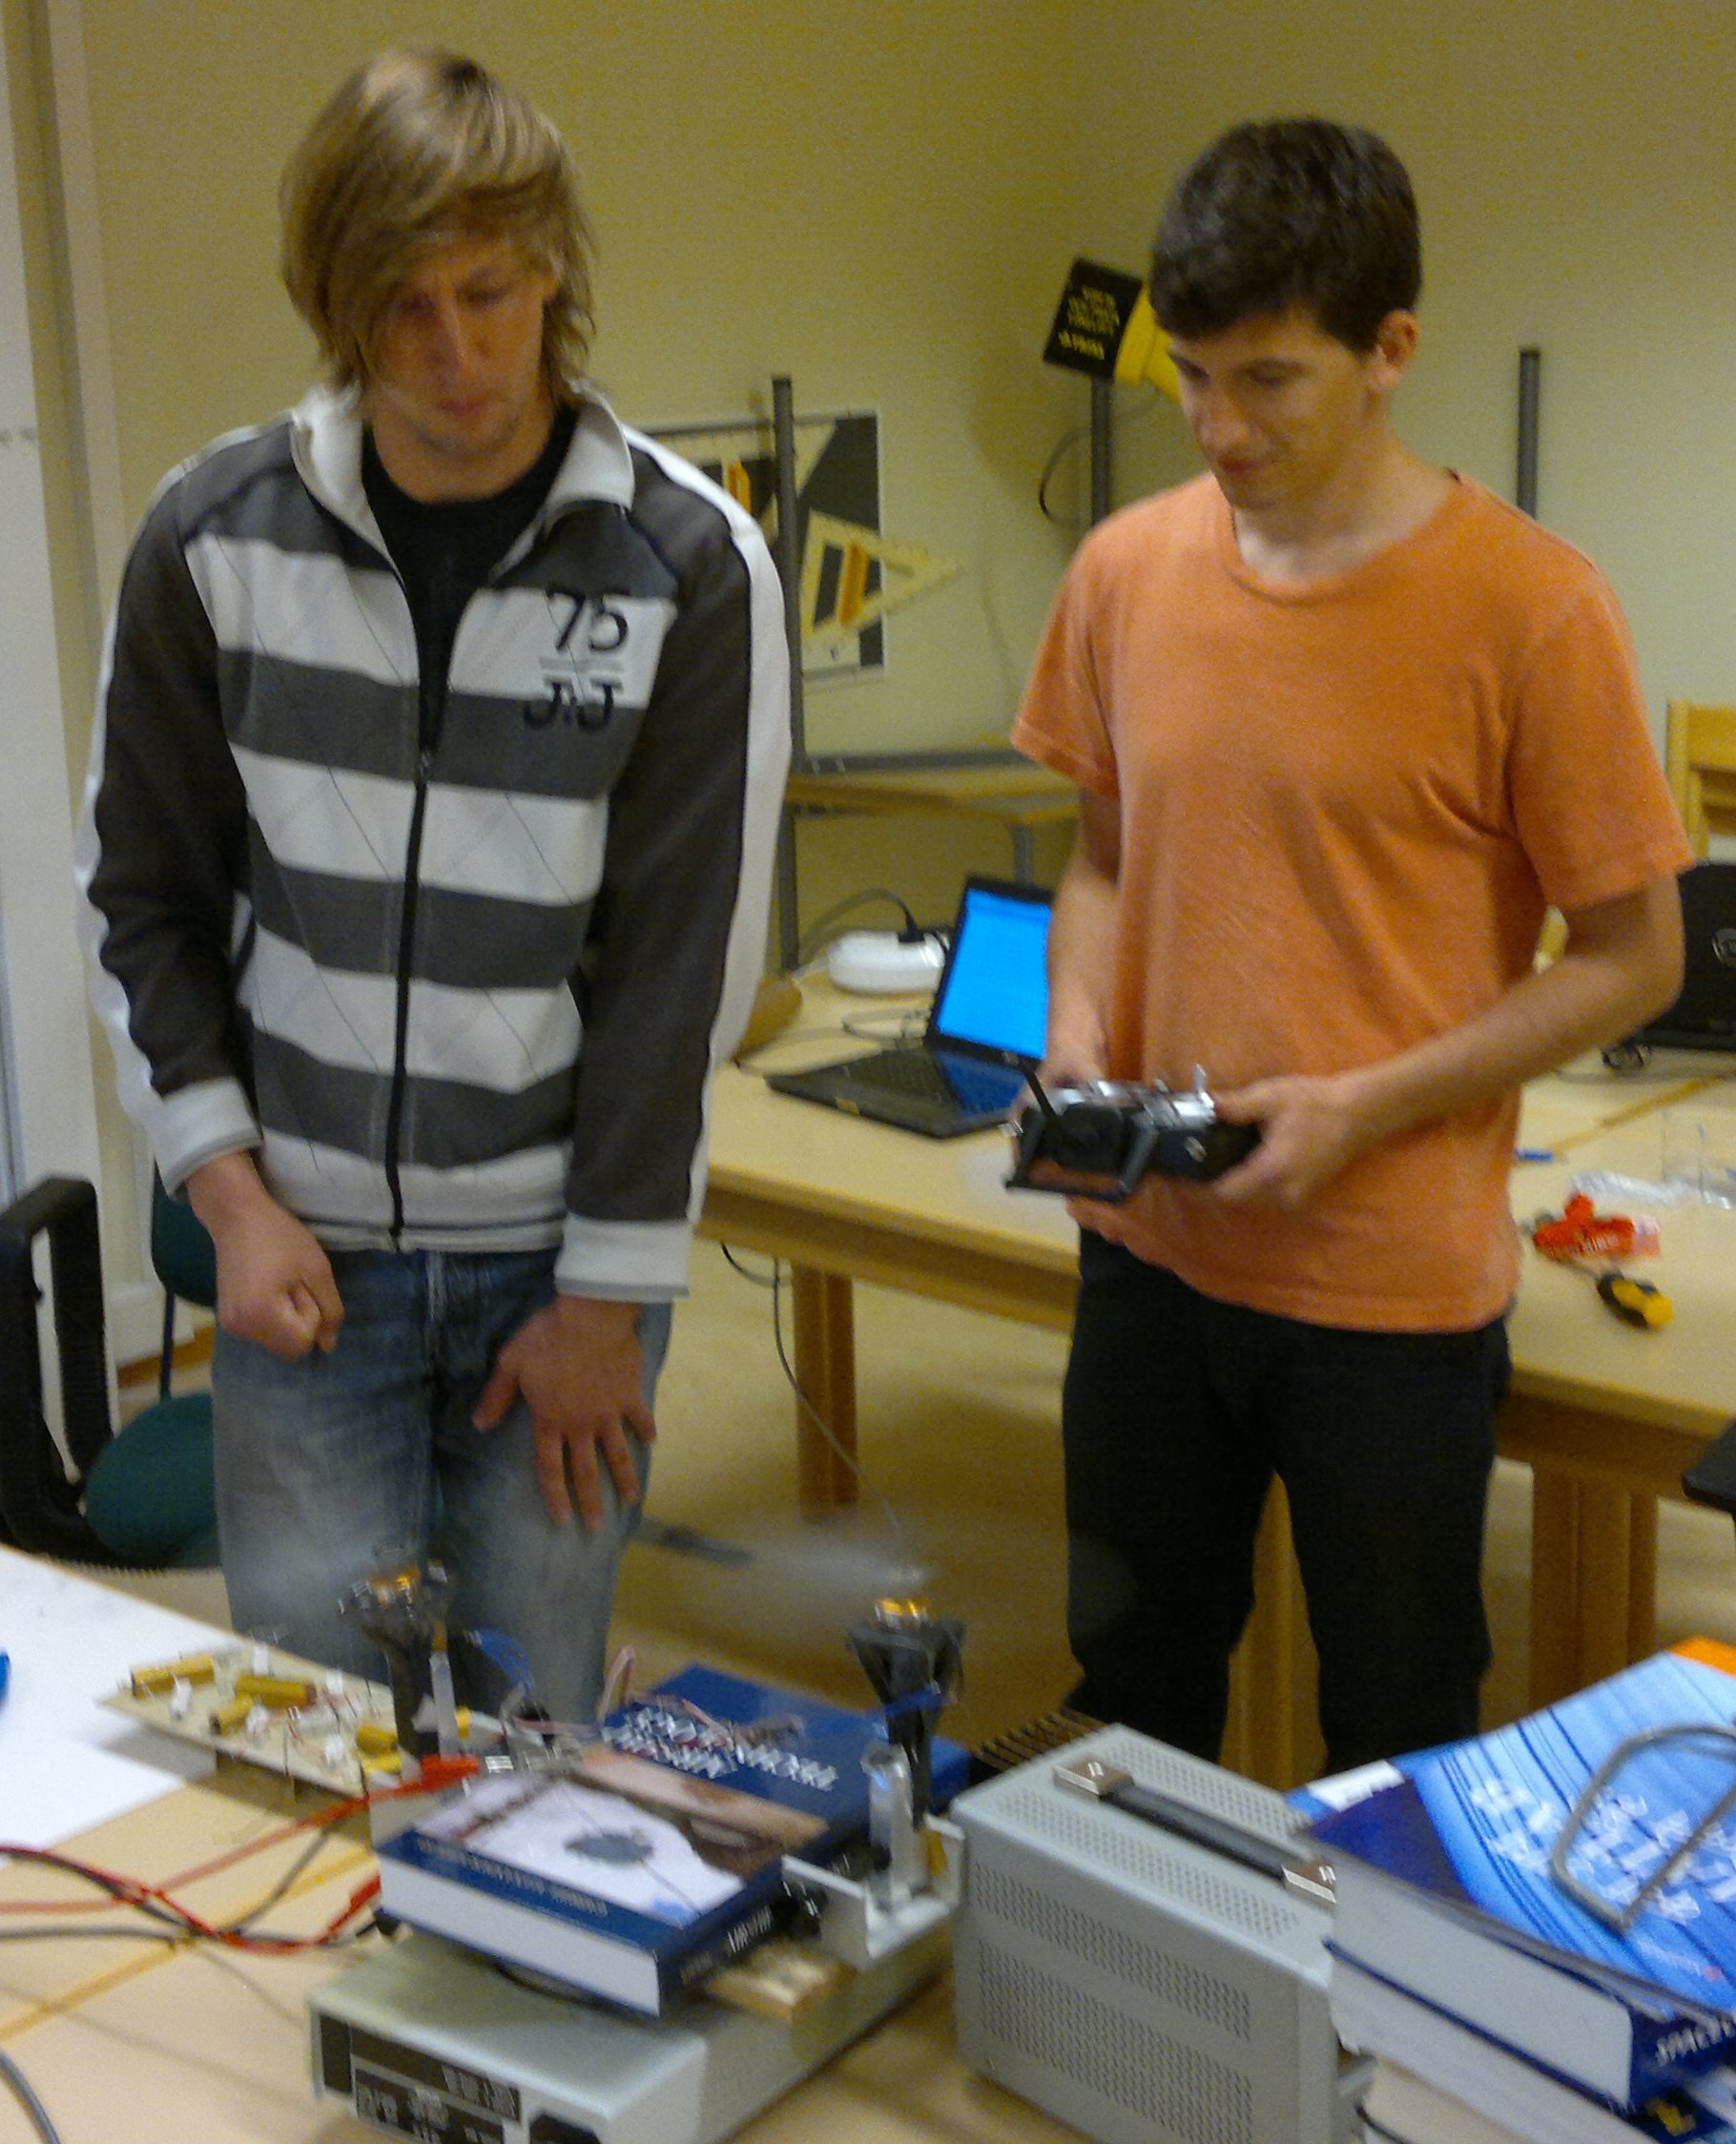
\includegraphics[scale=0.4]{figures/fig_CDR_MCC_motor_thrust_test2.jpg}
\end{minipage}
\caption{Stationary test of motor thrust level}
\label{fig:motor_thrust_level}
\end{figure}
%
%
\newpage
\section{Ressources}
%
Table \ref{tab:mcc_parts_list} list the ordered \ac{MCC} parts.
\begin{table}[bht]
\centering
\caption{MCC parts list}
\begin{tabular}{l l l}
\hline
\textbf{Part} &  \textbf{Part name} & \textbf{Supplier}\\ 
\hline
Motor & Turnigy $2204/14\;1450\,kv$ (AXI 2204) & \url{www.rcflight.se} \\
ESC & HobbyWing Flyfun $10\,A$, HW10A & \url{www.rcflight.se}\\
Propeller & APC Slowflyer Pusher $9 \times 4.7$ & \url{www.rcflight.se}\\
Transmitter & WFly WFT07 $2.4\,GHz$ 7-channels & \url{www.rcflight.se}\\
\hline
\end{tabular}
\label{tab:mcc_parts_list}
\end{table}
%